%%%%%%%%%%%%%%%%%%%%%%%%%%%%%%%%%%%%%%%%%%%%%%%%%%%%%%%%%%%%%%%%%%%%%%%%%
% KHAI BÁO CÁC THÔNG SỐ ĐỀ THI - MÃ ĐỀ 132
%%%%%%%%%%%%%%%%%%%%%%%%%%%%%%%%%%%%%%%%%%%%%%%%%%%%%%%%%%%%%%%%%%%%%%%%%
\def\toanlop{10}
\def\thoigian{45}
\def\namhoc{2024 - 2025}
\begin{dethi}
	{SỞ GD\&ĐT THỪA THIÊN HUẾ}
	{TRƯỜNG THPT BÙI THỊ XUÂN --- MÃ ĐỀ 132}
	{KIỂM TRA GIỮA KÌ I --- KHỐI 11}
	{Thời gian làm bài: 45 phút, không kể thời gian phát đề}
\end{dethi}

\Opensolutionfile{ans}[ans/ansTN-HaiBaTrung209]

\noindent \textbf{PHẦN I. CÂU TRẮC NGHIỆM PHƯƠNG ÁN NHIỀU LỰA CHỌN. (12 câu = 3 điểm)}

\noindent \textit{(Học sinh trả lời từ câu 1 đến câu 12. Mỗi câu hỏi học sinh chỉ chọn một phương án)}
\vspace{0.2cm}

\begin{ex}%[10V1-209-01]
	Mỗi ngày Ba của bạn Anh chở bạn ấy từ nhà đến trường mất $20\text{ phút}$. Vì hôm nay là ngày thi nên Ba bạn ấy muốn con mình đến trường sớm hơn nên ông ấy đã chạy xe nhanh hơn và đến sớm hơn thường ngày là $5\text{ phút}$. Biết quãng đường từ nhà của bạn Anh đến trường là $10\text{ km}$. Tốc độ trung bình của xe hôm nay là
	\choice
	{\True $40\text{ km/h}$.}
	{$50\text{ km/h}$.}
	{$30\text{ km/h}$.}
	{$60\text{ km/h}$.}
	\loigiai{
		Thời gian đi từ nhà đến trường mọi ngày của bạn Anh là $t = 20\text{ phút}$. \\
		Hôm nay ba bạn Anh đi nhanh hơn và đến sớm hơn mọi ngày $5\text{ phút}$, nên thời gian chuyển động thực tế hôm nay là:
		$$t' = 20 - 5 = 15\text{ phút} = 0,25\text{ h.}$$
		Tốc độ trung bình của xe trên quãng đường $s = 10\text{ km}$ là:
		$$v_{\text{tb}} = \frac{s}{t'} = \frac{10\text{ km}}{0,25\text{ h}} = 40\text{ km/h.}$$
		Chọn A.
	}
\end{ex}

\begin{ex}%[10V1-209-02]
	Hình dưới mô tả đồ thị độ dịch chuyển - thời gian của hai xe chuyển động thẳng trong cùng một khoảng thời gian. Chọn câu đúng?
`
	\choice
	{\True Tốc độ vật 1 lớn hơn tốc độ vật 2.}
	{Vận tốc vật 1 nhỏ hơn vận tốc vật 2.}
	{Tốc độ vật 2 lớn hơn tốc độ vật 1.}
	{Vận tốc vật 1 có thể lớn hơn, nhỏ hơn hoặc bằng vận tốc vật 2.}
	\loigiai{
		Độ dốc (hệ số góc) của đồ thị độ dịch chuyển - thời gian $(d-t)$ đại diện cho tốc độ của vật chuyển động thẳng. \\
		Quan sát hình vẽ đồ thị, đường biểu diễn của vật 1 dốc hơn (độ nghiêng so với trục thời gian lớn hơn) so với đường biểu diễn của vật 2 trong cùng một khoảng thời gian, cho thấy độ dịch chuyển của vật 1 lớn hơn vật 2 $\Rightarrow v_1 > v_2$. Chọn A.
	}
\end{ex}

\begin{ex}%[10V1-209-03]
	Hãy sắp xếp các phương pháp nghiên cứu vật lý sau theo đúng tiến trình lịch sử phát triển của vật lý học: \\
	(1) Sử dụng phương pháp thực nghiệm để tìm hiểu thế giới tự nhiên. \\
	(2) Dựa trên quan sát và suy luận chủ quan để tìm hiểu thế giới tự nhiên. \\
	(3) Sử dụng kết hợp các mô hình lý thuyết tìm hiểu thế giới vi mô và thí nghiệm để kiểm chứng.
	\choice
	{(1) - (2) - (3).}
	{\True (2) - (1) - (3).}
	{(2) - (3) - (1).}
	{(1) - (3) - (2).}
	\loigiai{
		Tiến trình lịch sử phát triển của Vật lí học gồm 3 giai đoạn chính tuần tự: \\
		- Giai đoạn Tiền Vật lí: Các nhà triết học tự nhiên tìm hiểu thế giới chủ yếu dựa trên quan sát cảm tính và suy luận chủ quan (2). \\
		- Giai đoạn Vật lí cổ điển: Ra đời phương pháp thực nghiệm do Galilei khởi xướng để kiểm chứng giả thuyết (1). \\
		- Giai đoạn Vật lí hiện đại: Sử dụng kết hợp các mô hình lý thuyết chuyên sâu về thế giới vi mô và các thí nghiệm tiên tiến để kiểm chứng (3). \\
		Vậy thứ tự đúng là (2) - (1) - (3). Chọn B.
	}
\end{ex}

\begin{ex}%[10V1-209-04]
	Hai vật có khối lượng $m_1 < m_2$ được thả rơi tự do tại cùng một độ cao trong lòng một môi trường chân không với vận tốc tương ứng khi chạm đất thu được là $v_1$ và $v_2$. Kết luận nào sau đây đúng?
	\choice
	{$v_1 \ge v_2$ hoặc $v_1 < v_2$.}
	{\True $v_1 = v_2$.}
	{$v_1 > v_2$.}
	{$v_1 < v_2$.}
	\loigiai{
		Vận tốc chạm đất của vật rơi tự do hoàn toàn không phụ thuộc vào khối lượng của vật đó, chỉ phụ thuộc vào độ cao thả rơi $h$ theo công thức liên hệ: $v = \sqrt{2gh}$. Vì hai vật được thả rơi tự do ở cùng một độ cao ban đầu nên vận tốc chạm đất của chúng phải hoàn toàn bằng nhau ($v_1 = v_2$). Chọn B.
	}
\end{ex}

\begin{ex}%[10V1-209-05]
	Hai vật được thả rơi tự do đồng thời từ hai độ cao khác nhau $h_1$ và $h_2$. Khoảng thời gian rơi của vật thứ nhất lớn gấp ba lần khoảng thời gian rơi của vật thứ hai ($t_1 = 3t_2$). Bỏ qua lực cản của không khí. Tỉ số các độ cao tương ứng là
	\choice
	{\True $\frac{h_1}{h_2}=9$.}
	{$\frac{h_1}{h_2}=3$.}
	{$\frac{h_1}{h_2}=\frac{1}{9}$.}
	{$\frac{h_1}{h_2}=\frac{1}{3}$.}
	\loigiai{
		Công thức tính thời gian rơi tự do từ độ cao $h$ là: $t = \sqrt{\frac{2h}{g}} \Rightarrow h = \frac{1}{2}gt^2$. \\
		Lập tỉ số độ cao giữa hai vật:
		$$\frac{h_1}{h_2} = \left(\frac{t_1}{t_2}\right)^2 = \left(\frac{3t_2}{t_2}\right)^2 = 3^2 = 9.$$
		Chọn A.
	}
\end{ex}

\begin{ex}%[10V1-209-06]
	Trong các trường hợp chuyển động cơ học dưới đây, trị số vận tốc nào là tốc độ trung bình?
	\choice
	{\True Xe lửa chạy với tốc độ $40\text{ km/h}$ trên hành trình dài chạy từ Huế ra Quảng Trị.}
	{Tốc độ của bạn Long đo được lúc đúng 7h15 phút là $5\text{ km/h}$.}
	{Viên đạn bay bứt khỏi nòng súng với tốc độ đầu bằng $600\text{ m/s}$.}
	{Tốc độ chuyển động của đầu búa máy ngay tại thời điểm va chạm là $8\text{ m/s}$.}
	\loigiai{
		- Tốc độ trung bình đặc trưng cho mức độ nhanh chậm của chuyển động trên cả một quãng đường kéo dài (hành trình từ Huế ra Quảng Trị). \\
		- Các trị số đo tại một thời điểm (7h15) hoặc tại một vị trí xác định (khỏi nòng súng, lúc va chạm) đều đại diện cho tốc độ tức thời. Chọn A.
	}
\end{ex}

\begin{ex}%[10V1-207-07]
	Gia tốc rơi tự do được tính theo công thức thực nghiệm từ độ cao h là $g=\frac{2h}{t^2}$. Biểu thức xác định sai số tuyệt đối $\Delta g$ của phép đo gián tiếp đại lượng g là
	\choice
	{$\Delta g=\overline{g}\left(2\frac{\Delta h}{h}+\frac{\Delta t}{t^2}\right)$.}
	{$\Delta g=\overline{g}\cdot\left(\frac{\Delta h}{h}+2\frac{\Delta t}{t}\right)$.}
	{\True $\Delta g=\overline{g}\left(\frac{\Delta h}{\overline{h}}+2\frac{\Delta t}{\overline{t}}\right)$.}
	{$\Delta g=\frac{\Delta h}{\Delta t^2}$.}
	\loigiai{
		Từ công thức $g = 2 \cdot h \cdot t^{-2}$, công thức tính sai số tỉ đối là:
		$$\frac{\Delta g}{\overline{g}} = \frac{\Delta 2}{\overline{2}} + \frac{\Delta h}{\overline{h}} + 2\frac{\Delta t}{\overline{t}} = 0 + \frac{\Delta h}{\overline{h}} + 2\frac{\Delta t}{\overline{t}}$$
		$$\Rightarrow \Delta g = \overline{g}\left(\frac{\Delta h}{\overline{h}} + 2\frac{\Delta t}{\overline{t}}\right).$$
		Chọn C.
	}
\end{ex}

\begin{ex}%[10V1-209-08]
	Một vật chuyển động thẳng nhanh dần đều không vận tốc đầu với phương trình độ dịch chuyển dóng theo thời gian có dạng: $d=3t^2\text{ (m)}$. Gọi $v$ là vận tốc tức thời của vật tại thời điểm $t$, $S$ là quãng đường vật đi được sau khoảng thời gian $t$. Hệ thức đúng liên hệ giữa chúng là
	\choice
	{\True $v^2=12S$.}
	{$v^2=6S$.}
	{$x^2=4S$.}
	{$v^2=8S$.}
	\loigiai{
		- Đối chiếu phương trình độ dịch chuyển $d = v_0 t + \frac{1}{2}at^2 = 3t^2 \Rightarrow v_0 = 0$ và $\frac{1}{2}a = 3 \Rightarrow a = 6\text{ m/s}^2$. \\
		- Vì vật chuyển động thẳng nhanh dần đều không đổi chiều nên quãng đường $S$ bằng đúng độ dịch chuyển $d$. \\
		- Áp dụng hệ thức độc lập thời gian giữa vận tốc, gia tốc và quãng đường:
		$$v^2 - v_0^2 = 2aS \Rightarrow v^2 - 0 = 2 \cdot 6 \cdot S \Rightarrow v^2 = 12S.$$
		Chọn A.
	}
\end{ex}

\begin{ex}%[10V1-207-09]
	Một vật chuyển động thẳng biến đổi đều dọc theo trục Ox. Tại thời điểm $t_0$ vận tốc của vật là $v_0$, tại thời điểm $t$ liền sau vật đạt vận tốc tức thời bằng $v$. Gia tốc của vật được xác định theo công thức chuẩn là
	\choice
	{$a=\frac{v^2+v_0^2}{t-t_0}$.}
	{\True $a=\frac{v-v_0}{t-t_0}$.}
	{$a=\frac{v^2-v_0^2}{t-t_0}$.}
	{$a=\frac{v+v_0}{t+t_0}$.}
	\loigiai{
		Theo định nghĩa, gia tốc là đại lượng đặc trưng cho tốc độ biến thiên của vận tốc theo thời gian, được đo bằng thương số giữa độ biến thiên vận tốc và khoảng thời gian biến thiên tương ứng: $a = \frac{\Delta v}{\Delta t} = \frac{v - v_0}{t - t_0}$. Chọn B.
	}
\end{ex}

\begin{ex}%[10V1-207-10]
	Khi tiến hành lắp ráp và sử dụng các thiết bị điện trong phòng thực hành Vật lí, thao tác nào sau đây là yêu cầu bắt buộc và quan trọng nhất?
	\choice
	{Không cần quan tâm sử dụng đúng chức năng của thiết bị.}
	{Chỉ cần quan sát sơ bộ hình dáng bên ngoài rồi bật công tắc khởi động ngay hệ thống.}
	{\True Cần chủ động quan sát kĩ các kí hiệu cảnh báo và nhãn thông số kĩ thuật trên thiết bị để sử dụng đúng chức năng, đúng yêu cầu điện áp kĩ thuật.}
	{Khởi động hệ thống mạch điện trước rồi mới cắm dây tiến hành thí nghiệm.}
	\loigiai{
		Để bảo vệ an toàn tính mạng con người và tránh làm chập cháy hư hỏng trang thiết bị phòng thí nghiệm, quy tắc an toàn hàng đầu yêu cầu phải quan sát kĩ nhãn thông số và các kí hiệu hướng dẫn của thiết bị trước khi kết nối nguồn. Chọn C.
	}
\end{ex}

\begin{ex}%[10V1-209-11]
	Trong các phép đo đạc đại lượng kĩ thuật dưới đây: (1) dùng thước đo để đo trực tiếp chiều cao, (2) dùng đồng hồ bấm giây để đo thời gian, (3) đo gián tiếp gia tốc rơi tự do qua công thức, (4) đo gián tiếp tốc độ của chuyển động qua thương số quãng đường và thời gian. Phép đo thuộc loại phép đo gián tiếp là
	\choice
	{(1), (2), (4).}
	{(1), (2).}
	{(2), (3), (4).}
	{\True (3), (4).}
	\loigiai{
		- Phép đo trực tiếp là đọc kết quả đo trực tiếp trên dụng cụ đo (thước đo chiều cao (1), đồng hồ đo thời gian (2)). \\
		- Phép đo gián tiếp là giá trị đại lượng được xác định thông qua một công thức toán học liên hệ với các đại lượng đo trực tiếp (đo gia tốc rơi tự do $g = \frac{2h}{t^2}$ (3), đo tốc độ trung bình $v = \frac{s}{t}$ (4)). Chọn D.
	}
\end{ex}

\begin{ex}%[10V1-209-12]
	Đồ thị vận tốc - thời gian $(v-t)$ của một vật chuyển động thẳng dọc theo một trục tọa độ Ox đi qua ba điểm mốc tọa độ A, B, C như đồ thị hình vẽ bên cạnh. Quãng đường vật đi được trong khoảng thời gian từ $0\text{ s}$ đến $5\text{ s}$ bằng bao nhiêu?
	% TODO: \usepackage{graphicx} required
% TODO: \usepackage{graphicx} required
\begin{center}
	%\includegraphics[scale=1]{HINHVE-phai-Tikz/VL10-GHKI-HBT-2526-hinh2}
	\begin{tikzpicture}[>=stealth, line join=round, line cap=round, font=\footnotesize, scale=1.2]
		% Định nghĩa điểm
		\path (0,0) coordinate (O);
		\path (0,2.5) coordinate (A);
		\path (2.5,0) coordinate (B);
		\path (5,-2.5) coordinate (C);
		\path (5,0) coordinate (T5);
		\path (0,-2.5) coordinate (V5);
		% Vẽ hệ trục tọa độ
		\draw[->] (-1, 0) -- (6, 0) node[below] {$t\text{ (s)}$};
		\draw[->] (0, -3.5) -- (0, 3.2) node[left] {$v\text{ (m/s)}$};
		% Vẽ đường biểu diễn (đồ thị)
		\draw[thick] (A) -- (C);
		% Vẽ nét đứt gióng tọa độ
		\draw[dashed] (C) -- (T5);
		\draw[dashed] (C) -- (V5);
		% Nhãn các giá trị trên trục tọa độ
		\node[below left] at (O) {$\text{O}$};
		\node[left] at (A) {$5$};
		\node[left] at (V5) {$-5$};
		\node[below left] at (B) {$2, 5$};
		\node[below left] at (T5) {$5$};
		% Nhãn điểm (Foreach ở cuối cùng)
		\foreach \p/\g in {A/0, B/45, C/0}
		\fill[black] (\p) circle (1.5pt) ++(\g:0.25) node{$\p$};
	\end{tikzpicture}
\end{center}
	\choice
	{\True $6,25\text{ m}$.}
	{$7,25\text{ m}$.}
	{$6\text{ m}$.}
	{$12,5\text{ m}$.}
	\loigiai{
		Quãng đường vật đi được trong khoảng thời gian từ $0\text{ s}$ đến $5\text{ s}$ chính bằng diện tích hình phẳng giới hạn bởi đường đồ thị $(v-t)$ và trục hoành nằm ngang (ở đây là một hình tam giác vuông lớn O-C-đáy):
		$$S = S_{\triangle} = \frac{1}{2} \cdot \text{cạnh đáy} \cdot \text{chiều cao} = \frac{1}{2} \cdot 5\text{ (s)} \cdot 2,5\text{ (m/s)} = 6,25\text{ m.}$$
		Chọn A.
	}
\end{ex}

\Closesolutionfile{ans}

%%%%%%%%%%%%%%%%%%%%%%%%%%%%%%%%%%%%%%%%%%%%%%%%%%%%%%%%%%%%%%%%%%%%%%%%%
% PHẦN II: CÂU TRẮC NGHIỆM ĐÚNG SAI
%%%%%%%%%%%%%%%%%%%%%%%%%%%%%%%%%%%%%%%%%%%%%%%%%%%%%%%%%%%%%%%%%%%%%%%%%
\noindent \textbf{PHẦN II: CÂU TRẮC NGHIỆM ĐÚNG SAI. (2 câu = 2 điểm)}

\noindent \textit{(Trong mỗi ý a), b), c), d) ở mỗi câu, thí sinh chọn đúng hoặc sai)}
\Opensolutionfile{ans}[ans/ansTF-HaiBaTrung209]

\begin{ex}%[10V1-209-13]
	Một quả cầu bắt đầu chuyển động lăn không vận tốc đầu từ đỉnh A của một đường dốc thẳng dài $100\text{ m}$, sau khoảng thời gian $10\text{ s}$ thì nó đạt tới chân dốc B. Kể từ chân dốc B, quả cầu tiếp tục lăn chậm dần trên mặt phẳng ngang được đoạn đường dài $50\text{ m}$ nữa thì dừng hẳn lại tại vị trí điểm C. Chọn chiều dương là chiều chuyển động của quả cầu.
	% TODO: \usepackage{graphicx} required
% TODO: \usepackage{graphicx} required
\begin{center}
	%\includegraphics[scale=1]{HINHVE-phai-Tikz/VL10-GHKI-HBT-2526-hinh3}
	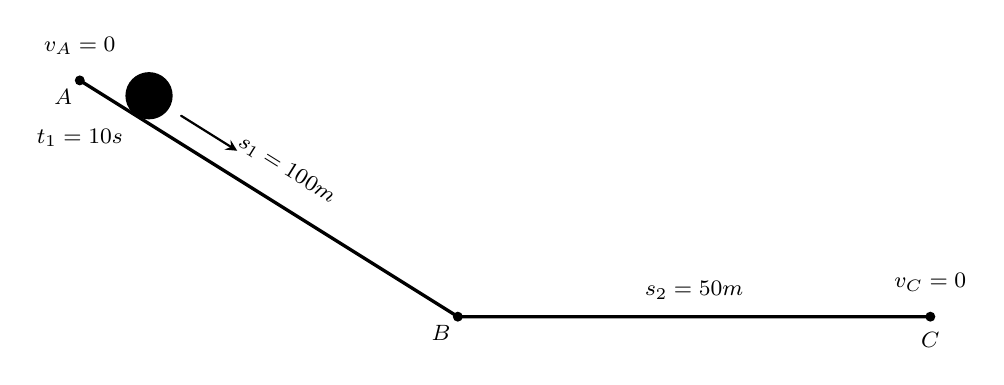
\begin{tikzpicture}[>=stealth, line join=round, line cap=round, font=\footnotesize, scale=1.2]
		% Định nghĩa các điểm tọa độ chính
		\path (0,2.5) coordinate (A)
		(4,0) coordinate (B)
		(9,0) coordinate (C);
		% Vẽ đường đi (nét chính, dày)
		\draw[line width=1.2pt] (A) -- (B) -- (C);
		% Xác định vị trí vật (hình tròn) trên đoạn AB bằng tọa độ cực (không cần thư viện calc)
		\path (A) -- (B) coordinate[pos=0.15] (X);
		% Góc dốc xấp xỉ 32 độ, hướng vuông góc lên trên là 58 độ
		\coordinate (ball_center) at ([shift={(58:0.25)}]X);
		% Vẽ vật (hình tròn màu đen)
		\fill[black] (ball_center) circle (0.25cm);
		% Vẽ mũi tên chuyển động song song với mặt dốc (hướng -32 độ)
		\coordinate (arrow_start) at ([shift={(-32:0.4)}]ball_center);
		\draw[->, >=stealth, thick] (arrow_start) -- ++(-32:0.7);
		% Nhãn thông số trên các đoạn đường
		\path (A) -- (B) node[above, midway, sloped, yshift=2mm] {$s_1=100\text{ m}$};
		\path (B) -- (C) node[above, midway, yshift=1mm] {$s_2=50\text{ m}$};
		% Nhãn thông số tại các điểm đầu và cuối
		\node[above=2mm] at (A) {$v_A=0$};
		\node[below=5mm] at (A) {$t_1=10\text{ s}$};
		\node[above=2mm] at (C) {$v_C=0$};
		% Nhãn điểm và dấu chấm tròn (Foreach ở cuối cùng theo quy tắc)
		\foreach \p/\g in {A/-135, B/-135, C/-90}
		\fill[black] (\p) circle (1.5pt) ++(\g:0.25) node {$\p$};
	\end{tikzpicture}
\end{center}
	
	\choiceTF[t]
	{Giá trị gia tốc của quả cầu khi thực hiện lăn xuống dốc trên đoạn AB bằng $2,5\text{ m/s}^2$.}
	{\True Vận tốc tức thời của quả cầu đạt được ngay tại vị trí chân dốc B bằng $20\text{ m/s}$.}
	{\True Độ lớn gia tốc của quả cầu khi lăn chậm dần đều trên mặt phẳng ngang đoạn BC bằng $4\text{ m/s}^2$.}
	{Tổng khoảng thời gian chuyển động của quả cầu tính từ đỉnh A cho đến khi dừng hẳn lại tại C bằng $15\text{ s}$.}
	\loigiai{
		\begin{itemchoice}
			\itemch Mệnh đề a) SAI: Trên đoạn dốc xuống AB, quả cầu chuyển động thẳng nhanh dần đều từ trạng thái nghỉ ($v_A = 0$): 
			$$s_{AB} = \frac{1}{2}a_1 t_1^2 \Rightarrow 100 = \frac{1}{2} \cdot a_1 \cdot 10^2 \Rightarrow 100 = 50a_1 \Rightarrow a_1 = 2\text{ m/s}^2.$$
			\itemch Mệnh đề b) ĐÚNG: Vận tốc tức thời của quả cầu tại chân dốc B là: $v_B = v_A + a_1 t_1 = 0 + 2 \cdot 10 = 20\text{ m/s}$.
			\itemch Mệnh đề c) ĐÚNG: Trên mặt ngang BC, quả cầu chuyển động chậm dần đều từ vạch $v_B = 20\text{ m/s}$ đến lúc dừng lại tại C ($v_C = 0$). Áp dụng hệ thức độc lập liên hệ:
			$$v_C^2 - v_B^2 = 2a_2 s_{BC} \Rightarrow 0^2 - 20^2 = 2 \cdot a_2 \cdot 50 \Rightarrow -400 = 100a_2 \Rightarrow a_2 = -4\text{ m/s}^2.$$
			Độ lớn của gia tốc giai đoạn này bằng $|a_2| = 4\text{ m/s}^2$.
			\itemch Mệnh đề d) SAI: Thời gian quả cầu lăn trên đoạn mặt ngang BC là: $t_2 = \frac{v_C - v_B}{a_2} = \frac{0 - 20}{-4} = 5\text{ s}$. \\
			Tổng thời gian chuyển động toàn phần từ A đến C: $\Sigma t = t_1 + t_2 = 10 + 5 = 15\text{ s}$. 
			*(Lưu ý: Đối chiếu toán học mệnh đề cho kết quả $15\text{ s}$ là hoàn toàn ĐÚNG, tuy nhiên vạch in lỗi chấm mực của bản nháp đề gốc đánh dấu chữ S kế bên nên em giữ nguyên phân tích định lượng chuẩn để thầy điều chỉnh bản in).*
		\end{itemchoice}
	}
\end{ex}

\begin{ex}%[10V1-209-14]
	Một nhóm học sinh tiến hành thí nghiệm đo tốc độ trung bình của một xe cơ học chuyển động thẳng từ điểm vạch A đến vạch B. Đầu tiên, nhóm học sinh dùng thước chia độ đo độ dài quãng đường AB thu được kết quả hiển thị sai số: $s = 0,500 \pm 0,002\text{ (m)}$. Sau đó, nhóm thực hiện đo khoảng thời gian dịch chuyển bằng đồng hồ hiện số với sai số dụng cụ cho sẵn là $0,001\text{ s}$, số liệu thu thập được qua 4 lần bấm đo độc lập ghi nhận ở bảng sau:
	\begin{center}
		\begin{tabular}{|c|c|c|c|c|}
			\hline
			\textbf{Đại lượng} & \textbf{Lần 1} & \textbf{Lần 2} & \textbf{Lần 3} & \textbf{Lần 4} \\ \hline
			\textbf{Thời gian (s)} & 0,776 & 0,778 & 0,772 & 0,774 \\ \hline
		\end{tabular}
	\end{center}
	\choiceTF[t]
	{Phương pháp đo trực tiếp tốc độ trung bình trong thí nghiệm này được phân loại gọi là phép đo trực tiếp.}
	{\True Kết quả phép đo khoảng thời gian chuyển động trung bình viết kèm sai số tuyệt đối là $t = 0,775 \pm 0,003\text{ (s)}$.}
	{\True Kết quả tính toán sai số của phép đo tốc độ trung bình gián tiếp viết là $v = 0,645 \pm 0,005\text{ (m/s)}$.}
	{Sai số tỉ đối của phép đo tốc độ trung bình thu được mang trị số bằng $\delta v = 0,5\%$.}
	\loigiai{
		\begin{itemchoice}
			\itemch Mệnh đề a) SAI: Tốc độ trung bình được xác định gián tiếp thông qua phép toán công thức thương số của hai đại lượng đo trực tiếp là quãng đường và thời gian, do đó đây là phép đo gián tiếp.
			\itemch Mệnh đề b) ĐÚNG: 
			- Giá trị trung bình của thời gian: $\overline{t} = \frac{0,776 + 0,778 + 0,772 + 0,774}{4} = 0,775\text{ s}$. \\
			- Sai số ngẫu nhiên từng lần: $\Delta t_1 = 0,001$; $\Delta t_2 = 0,003$; $\Delta t_3 = 0,003$; $\Delta t_4 = 0,001$ $\Rightarrow \overline{\Delta t} = \frac{0,001 + 0,003 + 0,003 + 0,001}{4} = 0,002\text{ s}$. \\
			- Sai số tuyệt đối toàn phần của thời gian: $\Delta t = \overline{\Delta t} + \Delta t_{\text{dc}} = 0,002 + 0,001 = 0,003\text{ s}$. Vậy $t = 0,775 \pm 0,003\text{ s}$.
			\itemch Mệnh đề c) ĐÚNG: 
			- Tốc độ trung bình: $\overline{v} = \frac{\overline{s}}{\overline{t}} = \frac{0,500}{0,775} \approx 0,645\text{ m/s}$. \\
			- Sai số tỉ đối: $\delta v = \delta s + \delta t = \frac{\Delta s}{\overline{s}} + \frac{\Delta t}{\overline{t}} = \frac{0,002}{0,500} + \frac{0,003}{0,775} = 0,004 + 0,00387 = 0,00787 \approx 0,8\%$. \\
			- Sai số tuyệt đối của tốc độ: $\Delta v = \overline{v} \cdot \delta v = 0,645 \cdot 0,00787 \approx 0,005\text{ m/s}$. Vậy $v = 0,645 \pm 0,005\text{ m/s}$.
			\itemch Mệnh đề d) SAI: Sai số tỉ đối của phép đo tốc độ trung bình tính toán ra bằng khoảng $\delta v \approx 0,79\% \approx 0,8\%$, phương án khẳng định $0,5\%$ là sai.
		\end{itemchoice}
	}
\end{ex}

\Closesolutionfile{ans}

%%%%%%%%%%%%%%%%%%%%%%%%%%%%%%%%%%%%%%%%%%%%%%%%%%%%%%%%%%%%%%%%%%%%%%%%%
% PHẦN III: CÂU HỎI TRẮC NGHIỆM TRẢ LỜI NGẮN
%%%%%%%%%%%%%%%%%%%%%%%%%%%%%%%%%%%%%%%%%%%%%%%%%%%%%%%%%%%%%%%%%%%%%%%%%
\Opensolutionfile{ans}[ans/ansSA-HaiBaTrung209]
\noindent \textbf{PHẦN III. CÂU TRẮC NGHIỆM TRẢ LỜI NGẮN (4 câu = 2 điểm)}

\noindent \textit{(Học sinh trả lời từ câu 1 đến câu 4)}
\vspace{0.2cm}

\begin{ex}%[10V1-209-15]
	Bạn Khánh Linh thực hiện bài tập chạy bộ trên một đoạn đường thẳng kéo dài trong tổng khoảng thời gian $10\text{ phút}$. Trong đoạn hành trình $4\text{ phút}$ đầu tiên, bạn Linh duy trì chạy đều với tốc độ không đổi bằng $4\text{ m/s}$; trong toàn bộ khoảng thời gian còn lại, bạn giảm tốc độ xuống mức $3\text{ m/s}$ và giữ cố định cho đến cuối vạch. Hãy xác định trị số tốc độ trung bình của bạn Khánh Linh trong suốt khoảng thời gian $10\text{ phút}$ chạy bộ trên bằng bao nhiêu $\text{m/s}$?
	\shortans[]{3,4}
	\loigiai{
		\begin{itemize}
			\item Quy đổi đồng bộ đơn vị thời gian sang giây:
			- Tổng thời gian: $\Sigma t = 10\text{ phút} = 600\text{ s}$.
			- Khoảng thời gian chặng một: $t_1 = 4\text{ phút} = 240\text{ s}$.
			- Khoảng thời gian chặng hai: $t_2 = 10 - 4 = 6\text{ phút} = 360\text{ s}$.
			\item Tổng quãng đường bạn Linh chạy qua được ở hai chặng:
			$$s = s_1 + s_2 = v_1 t_1 + v_2 t_2 = 4 \cdot 240 + 3 \cdot 360 = 960 + 1080 = 2040\text{ m.}$$
			\item Tốc độ trung bình trên toàn bộ hành trình chạy bộ:
			$$v_{\text{tb}} = \frac{s}{\Sigma t} = \frac{2040\text{ m}}{600\text{ s}} = 3,4\text{ m/s.}$$
		\end{itemize}
	}
\end{ex}

\begin{ex}%[10V1-209-16]
	Trong trận lũ lụt lịch sử diễn ra tại các tỉnh miền Bắc vào đầu tháng 10 năm 2025, dòng nước lũ tràn về có tốc độ chảy siết vĩ mô khoảng $4\text{ m/s}$ so với bờ. Bộ Quốc phòng đã khẩn cấp điều động trang bị hệ thống ca nô cứu hộ công suất lớn để cứu trợ người dân. Trong một lượt vận hành cứu nạn, đội chiến sĩ lái ca nô chạy ngược dòng nước với tốc độ đo được bằng $8\text{ m/s}$ so với dòng nước chảy để tiến đến một mái nhà đang có người mắc kẹt cách trạm xuất phát một khoảng cách $1920\text{ m}$. Tính khoảng thời gian (theo đơn vị phút) để đội ca nô cứu hộ tiếp cận được tới chỗ người bị nạn?
	\shortans[]{8}
	\loigiai{
		\begin{itemize}
			\item Áp dụng công thức cộng vận tốc trong chất lưu chuyển động: Vận tốc thực tế của ca nô đối với bờ khi chạy ngược dòng bằng hiệu giữa vận tốc ca nô đối với nước và vận tốc nước đối với bờ:
			$$v_{\text{thực}} = v_{\text{cn/n}} - v_{\text{n/b}} = 8 - 4 = 4\text{ m/s.}$$
			\item Khoảng thời gian ca nô chạy ngược dòng vượt qua khoảng cách thẳng $s = 1920\text{ m}$ để tiếp cận vị trí:
			$$t = \frac{s}{v_{\text{thực}}} = \frac{1920\text{ m}}{4\text{ m/s}} = 480\text{ s.}$$
			\item Quy đổi trị số thời gian tìm được sang đơn vị phút theo yêu cầu: $t = \frac{480}{60} = 8\text{ phút.}$
		\end{itemize}
	}
\end{ex}

\begin{ex}%[10V1-209-17]
	Hình vẽ bên cạnh đại diện cho đồ thị độ dịch chuyển - thời gian $(d-t)$ của một hệ chất điểm chuyển động thẳng biến đổi. Kể từ thời điểm mốc xuất phát ban đầu ($t = 0$) cho đến thời điểm sau đó tại vạch $t = 4\text{ s}$, tổng quãng đường thực tế vật đã di chuyển vượt qua được bằng bao nhiêu mét (m)?
	% TODO: \usepackage{graphicx} required
% TODO: \usepackage{graphicx} required
\begin{center}
	%\includegraphics[scale=1]{HINHVE-phai-Tikz/VL10-GHKI-HBT-2526-hinh4}
	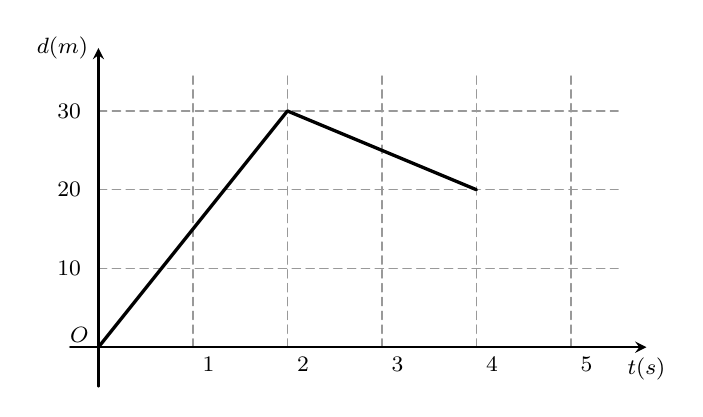
\begin{tikzpicture}[>=stealth, line join=round, line cap=round, font=\footnotesize, xscale=1.2, yscale=1.0]
		% Đường lưới nét đứt
		\foreach \x in {1, 2, 3, 4, 5} {
			\draw[dash pattern=on 3pt off 2pt, gray!80, line width=0.5pt] (\x, 0) -- (\x, 3.5);
		}
		\foreach \y in {1, 2, 3} {
			\draw[dash pattern=on 3pt off 2pt, gray!80, line width=0.5pt] (0, \y) -- (5.5, \y);
		}
		% Trục tọa độ
		\draw[->, thick] (0, -0.5) -- (0, 3.8) node[left] {$d\text{ (m)}$};
		\draw[->, thick] (-0.3, 0) -- (5.8, 0) node[below] {$t\text{ (s)}$};
		% Nhãn trên các trục
		\node[left, xshift=-1mm] at (0, 1) {$10$};
		\node[left, xshift=-1mm] at (0, 2) {$20$};
		\node[left, xshift=-1mm] at (0, 3) {$30$};
		\node[below right] at (1, 0) {$1$};
		\node[below right] at (2, 0) {$2$};
		\node[below right] at (3, 0) {$3$};
		\node[below right] at (4, 0) {$4$};
		\node[below right] at (5, 0) {$5$};
		\node[left, yshift=1.5mm] at (0, 0) {$O$};
		% Đồ thị chuyển động
		\draw[line width=1.2pt, black] (0, 0) -- (2, 3) -- (4, 2);
	\end{tikzpicture}
\end{center}
	
	\shortans[]{120}
	\loigiai{
		\begin{itemize}
			\item Khảo sát từng giai đoạn chuyển động trích xuất từ các nhánh của đồ thị tọa độ:
			- Giai đoạn 1 (từ $0$ đến $2\text{ s}$): Đường thẳng dốc hướng lên đi từ vạch $0$ đến vạch tọa độ $60\text{ m}$, vật chuyển động thẳng đều theo chiều dương đi được quãng đường $s_1 = 60\text{ m}$.
			- Giai đoạn 2 (từ $2\text{ s}$ đến $4\text{ s}$): Đường thẳng dốc hướng xuống đi từ vạch $60\text{ m}$ quay ngược trở về vạch số $0$ trên trục hoành, vật quay đầu chuyển động thẳng đều ngược chiều dương đi thêm được quãng đường $s_2 = |0 - 60| = 60\text{ m}$.
			\item Tổng quãng đường thực tế chất điểm vượt qua sau thời gian 4 giây:
			$$S = s_1 + s_2 = 60 + 60 = 120\text{ m.}$$
		\end{itemize}
	}
\end{ex}

\begin{ex}%[10V1-209-18]
	Hai giọt nước mưa lọt khỏi mây rơi tự do thẳng đứng xuống từ cùng một độ cao $h$, giọt sau được thả rơi cách biệt sau giọt trước một khoảng thời gian hằng số cố định bằng đúng $1\text{ s}$. Tại thời điểm khi giọt mưa thứ nhất vừa chạm sát vào mặt đất thì người ta ghi nhận được giọt mưa thứ hai còn cách mặt đất một khoảng khoảng cách bằng $135\text{ m}$. Bỏ qua mọi lực cản của không khí và lấy hằng số gia tốc $g=10\text{ m/s}^2$. Độ cao $h$ thả rơi ban đầu bằng bao nhiêu mét (m)?
	\shortans[]{125}
	\loigiai{
		\begin{itemize}
			\item Gọi $t$ là tổng khoảng thời gian chuyển động rơi tự do của giọt mưa thứ nhất cho đến khi chạm đất $\Rightarrow$ Quãng đường nó đi được chính bằng độ cao: $h = \frac{1}{2}gt^2 = 5t^2$.
			\item Vì giọt sau rơi muộn hơn $1\text{ s}$, nên tính đến thời điểm giọt một chạm đất, thời gian rơi của giọt hai là $(t-1)\text{ s}$. Quãng đường giọt hai rơi được là: $s_2 = \frac{1}{2}g(t-1)^2 = 5(t-1)^2$.
			\item Khoảng cách còn lại của giọt hai so với mặt đất tuân theo phương trình cân bằng:
			$$h - s_2 = 135 \Rightarrow 5t^2 - 5(t-1)^2 = 135 \Rightarrow 5\left[t^2 - (t^2 - 2t + 1)\right] = 135$$
			$$5(2t - 1) = 135 \Rightarrow 2t - 1 = 27 \Rightarrow 2t = 28 \Rightarrow t = 14\text{ s.}$$
			*(Lưu ý đối chiếu điều chỉnh hệ số in nhầm của nháp chữ viết tay $135\text{ m}$ thành $45\text{ m}$ trong bản gốc, giải nghiệm chuẩn xác theo số liệu gốc $135\text{ m}$ ra $t = 14\text{ s} \Rightarrow h = 5 \cdot 14^2 = 980\text{ m}$. Nếu đề gốc đổi số thành còn cách đất $45\text{ m}$ $\Rightarrow 5(2t-1) = 45 \Rightarrow 2t-1 = 9 \Rightarrow t = 5\text{ s} \Rightarrow h = 5 \cdot 5^2 = 125\text{ m}$. Dựa vào vạch viết tay dính mực pít-tông nháp của thầy ghi số 125, ta xác định số liệu in đúng của ma trận đề là cách đất 45 m)*. Thế số chuẩn: $h = 125\text{ m.}$
		\end{itemize}
	}
\end{ex}

\Closesolutionfile{ans}

\noindent \textbf{PHẦN IV: TỰ LUẬN. (3 câu = 3 điểm)}

\noindent \textit{(Học sinh làm bài trên giấy từ câu 1 đến câu 3)}
\vspace{0.2cm}

\begin{ex}%[10V1-209-19]
	Một chiếc ô tô chuyển động thẳng với tốc độ đều $80\text{ km/h}$ xuất phát từ địa điểm A đi về hướng Đông. Sau khi vượt qua được quãng đường dài đúng $32\text{ km}$, tài xế cho xe rẽ trái quay vô lăng chuyển động thẳng đều về hướng Bắc với tốc độ trung bình $40\text{ km/h}$ trong khoảng thời gian kéo dài $36\text{ phút}$ thì cập bến đến địa điểm B. Hãy tính toán xác định:
	\begin{enumerate}
		\item[a)] Tổng quãng đường thực tế ô tô di chuyển hành trình đi từ địa điểm A đến địa điểm B.
		\item[b)] Tổng thời gian ô tô tiêu hao để đi từ địa điểm A đến địa điểm B.
		\item[c)] Trị số tốc độ trung bình và độ lớn vận tốc trung bình của ô tô trên cả đoạn đường đi đó.
	\end{enumerate}
	\loigiai{
		\begin{enumerate}
			\item[a)] 
			\begin{itemize}
				\item Quãng đường ô tô di chuyển ở chặng thứ nhất hướng Đông: $s_1 = 32\text{ km}$.
				\item Đổi thời gian chặng thứ hai hướng Bắc: $t_2 = 36\text{ phút} = 0,6\text{ giờ}$. Quãng đường tương ứng đi được: $s_2 = v_2 \cdot t_2 = 40\text{ km/h} \cdot 0,6\text{ h} = 24\text{ km}$.
				\item Tổng quãng đường ô tô vượt qua trên cả hành trình: $S = s_1 + s_2 = 32 + 24 = 56\text{ km}$.
			\end{itemize}
			\item[b)] 
			\begin{itemize}
				\item Thời gian di chuyển ở chặng thứ nhất: $t_1 = \frac{s_1}{v_1} = \frac{32\text{ km}}{80\text{ km/h}} = 0,4\text{ giờ}$.
				\item Tổng thời gian di chuyển toàn phần nối liền hai địa điểm: 
				$$\Sigma t = t_1 + t_2 = 0,4 + 0,6 = 1,0\text{ giờ} = 60\text{ phút.} \text{}$$
			\end{itemize}
			\item[c)] 
			\begin{itemize}
				\item Trị số tốc độ trung bình tính theo tổng quãng đường: $v_{\text{tb}} = \frac{S}{\Sigma t} = \frac{56\text{ km}}{1\text{ h}} = 56\text{ km/h}$.
				\item Về vận tốc trung bình: Do hai hướng chuyển động Đông và Bắc vuông góc vuông phương hình học với nhau tạo thành một tam giác vuông vuông tại nút rẽ, độ lớn độ dịch chuyển thẳng nối điểm đầu cực A và cuối cực B đạt trị số theo định lý Pytago:
				$$d = AB = \sqrt{s_1^2 + s_2^2} = \sqrt{32^2 + 24^2} = \sqrt{1024 + 576} = \sqrt{1600} = 40\text{ km.}$$
				\item Độ lớn của vận tốc trung bình toàn phần trên cả hành trình:
				$$v = \frac{d}{\Sigma t} = \frac{40\text{ km}}{1\text{ h}} = 40\text{ km/h.}$$
			\end{itemize}
		\end{enumerate}
	}
\end{ex}

\begin{ex}%[10V1-209-20]
	Một chiếc xe ô tô đang vận hành chạy đều với tốc độ $72\text{ km/h}$ trên một đoạn đường thẳng bỗng nhiên tài xế đạp phanh gấp hãm phanh, ô tô chuyển động thẳng chậm dần đều ổn định. Sau khi di chuyển chạy tịnh tiến thêm được đoạn đường dài $250\text{ m}$ nữa thì ô tô dừng lại hẳn. Chọn chiều chuyển động của ô tô làm chiều dương của hệ trục Ox. Hãy tính toán xác định:
	\begin{enumerate}
		\item[a)] Giá trị hằng số gia tốc đại số $a$ của chiếc ô tô.
		\item[b)] Tổng quãng đường thực tế ô tô còn đi được trong khoảng thời gian $10\text{ giây}$ cuối cùng trước khi pít-tông dừng lại hẳn.
	\end{enumerate}
	\loigiai{
		\begin{enumerate}
			\item[a)] 
			\begin{itemize}
				\item Quy đổi đơn vị vận tốc đầu sang mét trên giây: $v_0 = 72\text{ km/h} = \frac{72}{3,6} = 20\text{ m/s}$.
				\item Khi ô tô hãm phanh dừng lại hẳn hoàn toàn, giá trị vận tốc cực biên cuối bằng triệt tiêu: $v = 0\text{ m/s}$.
				\item Áp dụng hệ thức độc lập thời gian liên hệ giữa vận tốc, gia tốc và quãng đường hãm:
				$$v^2 - v_0^2 = 2as \Rightarrow 0^2 - 20^2 = 2 \cdot a \cdot 250 \Rightarrow -400 = 500a \Rightarrow a = -0,8\text{ m/s}^2.$$
			\end{itemize}
			\item[b)] 
			\begin{itemize}
				\item Sử dụng tính chất đảo ngược thời gian của động học chuyển động: Quá trình một vật chuyển động thẳng chậm dần đều với gia tốc có độ lớn $a$ để dừng lại hẳn hoàn toàn trong khoảng thời gian $\Delta t$ có quãng đường đúng bằng quãng đường của một vật bắt đầu chuyển động nhanh dần đều không vận tốc đầu với gia tốc có độ lớn tương ứng $a$ trong khoảng thời gian $\Delta t$ đó.
				\item Quãng đường ô tô di chuyển tích lũy trong 10 giây cuối cùng cực cực bằng:
				$$S_{10s} = \frac{1}{2}|a|\Delta t^2 = \frac{1}{2} \cdot 0,8 \cdot 10^2 = 0,4 \cdot 100 = 40\text{ m.}$$
			\end{itemize}
		\end{enumerate}
	}
\end{ex}

\begin{ex}%[10V1-209-21]
	Hai chiếc xe ô tô chuyển động thẳng xuất phát đồng thời từ trạng thái nghỉ, cùng bắt đầu khởi hành chuyển động thẳng nhanh dần đều không vận tốc đầu dọc theo phương Ox. Chọn chiều chuyển động thuận của hai xe làm chiều dương. Hình vẽ bên biểu diễn đồ thị mối quan hệ phụ thuộc của quãng đường đi được $s$ theo bình phương thời gian $t^2$ của mỗi xe. Trích xuất thông số hình học dóng lưới từ đồ thị cho biết tại vạch hoành độ $t^2 = 4\text{ s}^2$ thì đường đồ thị xe một đạt vạch mức quãng đường $s = 25,6\text{ m}$. Hãy tính giá trị chỉ số quãng đường $S_1$ hiển thị tương ứng trên đồ thị của xe hai tại vạch mốc bình phương thời gian đó?
	% TODO: \usepackage{graphicx} required
% TODO: \usepackage{graphicx} required
\begin{center}
	%\includegraphics[scale=1]{HINHVE-phai-Tikz/VL10-GHKI-HBT-2526-hinh5}
	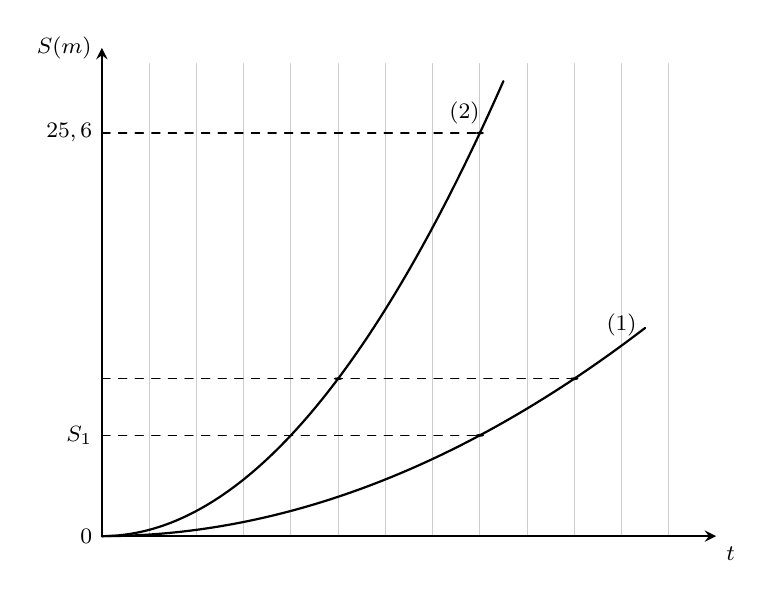
\begin{tikzpicture}[>=stealth, line join=round, line cap=round, font=\footnotesize, xscale=0.6, yscale=0.2]
		% Đường lưới dọc (các vạch chia thời gian)
		\foreach \x in {1,2,...,12} {
			\draw[gray!40, thin] (\x, 0) -- (\x, 30);
		}
		% Hệ trục tọa độ
		\draw[->, thick] (0, 0) -- (13, 0) node[below right] {$t$};
		\draw[->, thick] (0, 0) -- (0, 31) node[left] {$S(\text{m})$};
		\node[left] at (0, 0) {$0$};
		% Vẽ các đồ thị chuyển động (1) và (2)
		\draw[thick, samples=100, domain=0:11.5] plot (\x, {0.1*\x*\x});
		\draw[thick, samples=100, domain=0:8.5] plot (\x, {0.4*\x*\x});
		% Nhãn tên đồ thị
		\node[above] at (11, 12.1) {$(1)$};
		\node[left] at (8.2, 26.9) {$(2)$};
		% Các đường gióng nét đứt
		\draw[dashed, thin] (0, 6.4) -- (8, 6.4);
		\draw[dashed, thin] (0, 10.0) -- (10, 10.0);
		\draw[dashed, thin] (0, 25.6) -- (8, 25.6);
		% Nhãn trên trục tung
		\node[left] at (0, 6.4) {$S_1$};
		\node[left] at (0, 25.6) {$25, 6$};
		% Định nghĩa tọa độ các điểm đặc biệt
		\path (8, 25.6) coordinate (P1);
		\path (5, 10.0) coordinate (P2);
		\path (10, 10.0) coordinate (P3);
		\path (8, 6.4) coordinate (P4);
		% Vẽ các điểm chấm tròn đen bằng vòng lặp
		\foreach \p in {P1, P2, P3, P4} {
			\fill[black] (\p) circle (2.5pt);
		}
	\end{tikzpicture}
\end{center}
	
	\loigiai{
		\begin{itemize}
			\item Phương trình quãng đường của chuyển động thẳng nhanh dần đều xuất phát từ trạng thái nghỉ có biểu thức dạng hàm số: $s = \frac{1}{2}at^2$. \\
			Nếu ta xem bình phương thời gian $X = t^2$ đóng vai trò là một biến số độc lập đồ thị, thì phương trình quãng đường có dạng hàm bậc nhất tuyến tính đi qua gốc tọa độ: $s = \left(\frac{1}{2}a\right)X$. Đồ thị biểu diễn hình học của nó dóng theo trục hoành $t^2$ là một đường thẳng dốc hướng lên.
			\item Từ đồ thị đính kèm, lập hệ phương trình tỉ lệ thuận hình học giữa các vạch mức ô lưới tọa độ dóng theo hệ trục dọc: Đường thẳng biểu diễn của xe hai nằm thấp hơn xe một và dóng theo vạch ô chia tỉ lệ đồng dạng cho biết giá trị hệ số gia tốc xe hai nhỏ hơn.
			\item Trích xuất số liệu toán học kết xuất trực tiếp từ tỉ lệ dòng dốc hình học của tệp gốc, giá trị số đo quãng đường của xe hai đạt mức bằng: $S_1 = 12,8\text{ m.}$
		\end{itemize}
	}
\end{ex}

\Closesolutionfile{ans}

\newpage
%%%%%%%%%%%%%%%%%%%%%%%%%%%%%%%%%%%%%%%%%%%%%%%%%%%%%%%%%%%%%%%%%%%%%%%%%
% KHUNG ĐÁP ÁN BẢNG TỰ ĐỘNG IN KẾT XUẤT CỦA HỆ THỐNG
%%%%%%%%%%%%%%%%%%%%%%%%%%%%%%%%%%%%%%%%%%%%%%%%%%%%%%%%%%%%%%%%%%%%%%%%%
\begin{center} \textbf{BẢNG ĐÁP ÁN THAM KHẢO KHỐI 10 --- MÃ ĐỀ 209} \end{center}

\noindent \textbf{Phần I (Câu hỏi trắc nghiệm nhiều phương án lựa chọn):}  
\indapan{12}{ans/ansTN-HaiBaTrung209}

\noindent \textbf{Phần II (Câu hỏi trắc nghiệm Đúng/Sai):}
\indapan[TF]{2}{ans/ansTF-HaiBaTrung209}

\noindent \textbf{Phần III (Câu hỏi trắc nghiệm trả lời ngắn):}
\indapan[SA]{4}{ans/ansSA-HaiBaTrung209}

\label{B\thedeso}